\thispagestyle{plain}
Generating a depth map from a pair of stereo cameras involves 3 main steps.  First, each camera must be calibrated, a process that removes distortion and calculates several parameters useful in the later steps.  Second, the cameras must be rectified, which translates, rotates and skews the images such that the cameras appear to exist on the same plane.  Lastly, the images are then processed using a stereo block matching algorithm to find corresponding areas in each of the images.  From this correspondence, depth values can be estimated and written into a depth map.

\section{Calibration}
In order to calibrate a single camera, several things must be calculated.  These values are referred to as the Intrinsic and Extrinsic parameters of the camera.  The Intrinsic parameters of a camera relate the image coordinates to the Idealized image coordinates and correct for the "Skewness" of the image. The Extrinsic parameters of a camera calculate the cameras position with respect to some general frame of reference.


\subsection{Intrinsic Parameters}

\begin{figure}[h!]
\begin{center}
  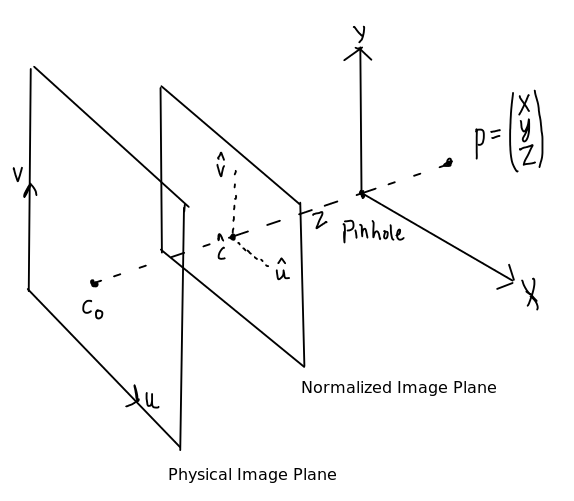
\includegraphics[scale=.5]{Image1}
  \caption{Pinhole Camera Model}
  \label{fig:Pinhole}
\end{center}
\end{figure}


Consider Figure \ref{fig:Pinhole}, where $x$ and $y$ refer to a single position in "world space", $\hat{u}$ and $\hat{v}$ refer to that same position on the normalized image plane, and $u$ and $v$ refer to that position on the physical image plane.  This is what is known as the "Pinhole Camera Model", as all points on the physical image plane can be thought of as having been projected through a point of size 0 existing somewhere in worldspace.  One thing to note here is that $\hat{u}$ and $\hat{v}$ can be calculated by $x/z$ and $y/z$ respectively.
\subsubsection{Skew}
The first calculation of the intrinsic camera parameters deals with the "skew" of the image.  As can be observed in Figure \ref{fig:Skew}, the physical image plane may not be a perfect rectangle.  Due to defects in craftmanship and/or wear and tear on the camera, the physical image plane may be a parallelogram.  In this case, x and y can be related to u and v via the calculation of $u=\hat{u}-\frac{y}{z} * \frac{sin  \theta }{ cos \theta} * f$ and $v=\hat{v}*\frac{1}{sin \theta} * f$ respectively, where $\theta$ is the angle between the perpendicular axis and the observed axis and $f$ is the focal length of the camera.
\begin{figure}[h!]
\begin{center}
	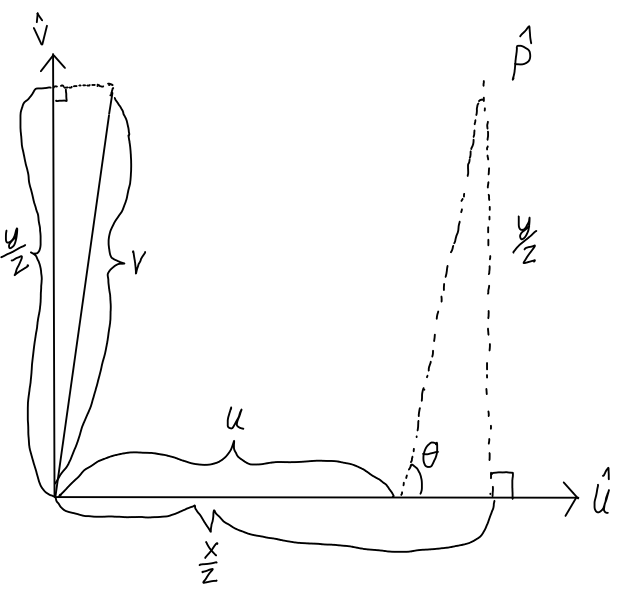
\includegraphics[scale=.5]{Image2}
	\caption{Image Skew}
	\label{fig:Skew}
\end{center}
\end{figure}
In addition to the physical image plane not being rectangular, it may also not be aligned with the idealized image plane.  To
account for this 2 new values, $u_0$ and $v_0$, are introduced to account for this misalignment.  This means that the
calculation becomes $u=\hat{u}-\frac{y}{z} * cot \theta * f + u_0$ and $v=\hat{v} * \frac{1}{sin \theta} * f + 
v_0$. By substituting $\alpha$ and $\beta$ for the horizontal and vertical focal length, these formulas can be rewritten as a 
multiplication of homogenous coordinates, like so $\begin{bmatrix} u \\ v \\ 1 \end{bmatrix} = \begin{bmatrix} \alpha & -\alpha 
cot\theta & u_{0} \\ 0 & \frac{\beta}{sin\theta} & v_{0} \\ 0 & 0 & 1 \end{bmatrix} \begin{bmatrix}\hat{u} \\ \hat{v}\\ 
1\end{bmatrix}$.  
Now, recalling that $u$ and $v$ refer to points on the actual image ($p$) and $\hat{u}$ and $\hat{v}$ refer to that same point 
on the normalized image plane ($\hat{p}$), then the matrix $\begin{bmatrix} \alpha & -\alpha cot\theta & u_0 \\ 0 & \frac{\beta}
{sin\theta} & v_0 \\ 0 & 0 & 1 \end{bmatrix}$ can be interpreted as a transformation matrix between points on the normalized image 
plane into points on the actual image.  This matrix is reffered to as $K$ from here on out.  Recalling that $\hat{p}$ refers to 
the column vector $\begin{bmatrix} \hat{u} \\ \hat{v} \\ 1 \end{bmatrix}$ and that $\hat{u} = \frac{x}{z}$ and $\hat{v} = \frac{y}
{z}$, $\hat{p}$ can be written as $\begin{bmatrix} \frac{x}{z} \\ \frac{y}{z} \\ 1 \end{bmatrix}$.  This can be then be decomposed into the matrix multiplication $\begin{bmatrix} \frac{1}{z} & 0 & 0 & 0 \\ 0 & \frac{1}{z} & 0 & 0 \\ 0 & 0 & \frac{1}{z} & 0 
\end{bmatrix} * \begin{bmatrix} x \\ y \\ z \\ 1 \end{bmatrix}$.  Furthermore, $\frac{1}{z}$ can be pulled out of the matrix multiplication 
resulting in $\frac{1}{z}\bigg[ I_{3x3} 0_{3x1} \bigg]P$.  This can then be substituted into the previous formula such that $p 
= K * \frac{1}{z}\bigg[I_{3x3}0_{3x1}\bigg] * P = \frac{1}{z}\bigg[K0\bigg]_{3x4}*P$.  Therefore the transformation from world 
coordinates $P$ to image coordinates $p$ can be written as $\frac{1}{z}MP$.  $M$ is referred to as the "Projection Matrix" from here 
on out.

\subsection{Extrinsic Parameters}
The Extrinsic parameters of the camera can be defined as the Location and Pose of the camera with respect to some reference frame.  The reference frame can be defined via the vectors $\vec{i}$, $\vec{j}$ and $\vec{k}$ which are orthoganal unit vectors making up the base of the "universal frame".  Using these vectors a pair of coordinate systems, $\{a\}$ and $\{b\}$, can defined by $O_a$,$\vec{i_a}$, $\vec{j_a}$ and $\vec{k_a}$ with $O_a$ defining the origin and $\vec{i_a}$, $\vec{j_a}$ and $\vec{k_a}$ defining the basis vectors.  Given these two new coordinate systems, a rotation and translation matrix can be generated that gives us the cameras location in worldspace.

\section{Rectification}
Once each of the Stereo cameras has been calibrated, they must then be rectified.  Rectification is the process by which the images from each camera are rotated and skewed so as to bring the images into the same image plane.

\subsection{Epipolar Geometry}
Before discussing how rectification works, it is useful to discuss the concept of epipolar geometry.  Recalling that the camera model considers each point on the image plane to have been projected through a size-zero point existing in worldspace, then a ray can be un-projected from the image pixel back through that point into infinity.  Then, every point on that ray can be projected through the focal point of the second camera. The resulting set of points on the image plane are referred to as Epipolar Lines, and the point where all of these epipolar lines converge is refered to as the epipole.  This holds true for each point in the second image as well, as they will correspond to epipolar lines in the first image.

\subsection{Rectification}
Rectification involves building a transform for each camera such that them images fall into the same image plane.  To restate using the previous definitions of epipolar geometry, Rectification generates a transform for each camera head such that the epipoles of both images exist at infinity and the epipolar lines in both images are parallel.  This is done by first creating a new coordinate system consisting of 3 unit vectors$e_1, e_2$ and $e_3$. The vector $e_1$ is generated by normalizing the epipole.  Since the image center is treated as the origin, $e_1$ is calculated by $\frac{T}{||T||}$ (T is the translation between the cameras, which was calculated in the calibration step).  $e_2$ is only constrained by the fact that it must be orthoganal to $e_1$ so it is generated by calculating the cross product of $e_1$ with the optical center.  $e_3$ is calculated by the cross product of $e_1$ and $e_2$.  Given these 3 vectors, $R_{rect}$ is calculated as $\begin{bmatrix} e_1^T \\ e_2^T \\ e_3^T \end{bmatrix}$.  This matrix rotates the first image around the optical center such that the epipolar lines become horizontal.  The matrices $R_l= R_rect$ and $R_r = R(R_rect)$ are then defined, with R being the rotation between the cameras that was calculated in the calibration step.  Now, for each point in the first image $p_1 = [x, y, f]^T$, the calculation $R_lp_1 = [x'y'z']$ is performed and the coordinates of the corresponding point in the new image are defined as $P_l' = \frac{f}{z}[x',y',z']$.  This step is then repeated with $R_r$ and points in the second image.


\section{Correspondence}
Once the images are rectified, It is time to calculate the correspondence.  This is by far the most computationally expensive portion of this process.  The algorithm is as follows:  For each pixel in the first image, search along its epipolar line in the second image until a "matching" pixel is found.  Compare the coordinates of the two pixels to calculate the distance between the apparent locations in the images. The resulting disparity value can be used to calculate the distance of that particular pixel from the camera.  Because the images are rectified, the search is constrained to the same scanline or y coordinate of the pixel in the second image, and only the X coordinate need be considered when calculating the disparity.  A pixel is "matching".  There are several techniques for calculating this, But both involve a "Sliding Window" that takes into account the pixels surrounding the target pixel.  This sliding window is moved along the scanline in the second image and the results are compared to the same sized window surrounding the source pixel.  Two of the techniques for comparing these windows are the Sum of Absolute Differences (SAD) and the Sum of Squared Differences (SSD).  In both of these techniques, each pixel in the target is subtracted from the same pixel in the source.  In SAD, the absolute value of this result is taken, and in SSD it is squared.  The results for all of the pixels in the current window is then summed, and compared against the previous minimum.  When the sliding window reaches the end of the scanline or the minimum reaches 0, the x coordinate of the target pixel is compared against the x coordinate of the source pixel, resulting in the disparity between the points.  If the relative positioning of the cameras is known beforehand, this correspondence search can be optimized by only searching along the portion of the scanline that might contain the pixel.  For example, if it is known that the source image has been taken by the left camera and the target by the right, then it would make little sense to search along the portions of the target image with a larger x coordinate than that of the source image.